\documentclass[border=4pt]{standalone}
\usepackage{fontspec}
\usepackage{amsmath}
\usepackage{unicode-math}
\setmainfont{Latin Modern Roman}
\setmathfont{Latin Modern Math}
\usepackage{pgfplots}
\usepackage{pgfplotstable}
\pgfplotsset{compat=1.18}
\usepackage{tkz-euclide}
\usetikzlibrary{arrows.meta,calc,angles,quotes,patterns,3d,backgrounds}
\definecolor{ink}{HTML}{123428}
\definecolor{asy}{HTML}{475569}
\definecolor{mint}{HTML}{86e0bd}
\tikzset{asym/.style={asy, line width=0.9pt, dash pattern=on 5pt off 3.5pt},
         guide/.style={gray!70, line width=0.6pt, densely dotted},
         dot/.style={circle, inner sep=0pt, minimum size=5pt, draw=white, line width=0.5pt},
         odot/.style={circle, inner sep=0pt, minimum size=5.5pt, fill=white, line width=1pt},
         lab/.style={font=\footnotesize, inner sep=1.5pt, text=ink}}
\begin{document}
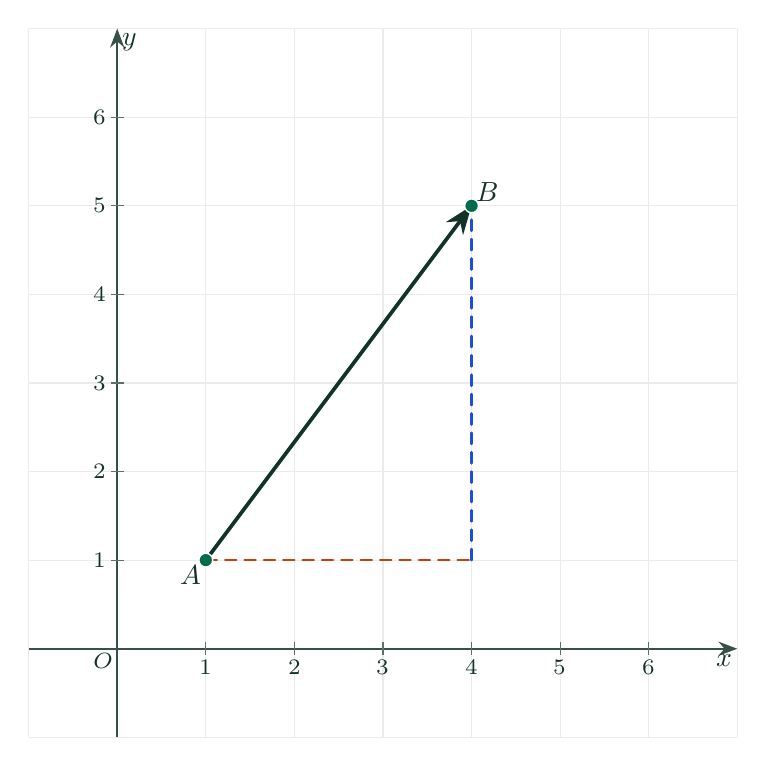
\begin{tikzpicture}[x=1.1250cm, y=1.1250cm]
\draw[gray!16, line width=0.4pt] (-1,-1) -- (-1,7) (0,-1) -- (0,7) (1,-1) -- (1,7) (2,-1) -- (2,7) (3,-1) -- (3,7) (4,-1) -- (4,7) (5,-1) -- (5,7) (6,-1) -- (6,7) (7,-1) -- (7,7);
\draw[gray!16, line width=0.4pt] (-1,-1) -- (7,-1) (-1,0) -- (7,0) (-1,1) -- (7,1) (-1,2) -- (7,2) (-1,3) -- (7,3) (-1,4) -- (7,4) (-1,5) -- (7,5) (-1,6) -- (7,6) (-1,7) -- (7,7);
\draw[ink!85, line width=0.7pt, -{Stealth[length=2.4mm]}] (-1,0) -- (7,0) node[anchor=north east, lab, font=\normalsize] {$x$};
\draw[ink!85, line width=0.7pt, -{Stealth[length=2.4mm]}] (0,-1) -- (0,7) node[anchor=north west, lab, font=\normalsize] {$y$};
\draw[ink!70] (1,0.07111111111111111) -- (1,-0.07111111111111111) node[below, lab, font=\footnotesize] {$1$};
\draw[ink!70] (2,0.07111111111111111) -- (2,-0.07111111111111111) node[below, lab, font=\footnotesize] {$2$};
\draw[ink!70] (3,0.07111111111111111) -- (3,-0.07111111111111111) node[below, lab, font=\footnotesize] {$3$};
\draw[ink!70] (4,0.07111111111111111) -- (4,-0.07111111111111111) node[below, lab, font=\footnotesize] {$4$};
\draw[ink!70] (5,0.07111111111111111) -- (5,-0.07111111111111111) node[below, lab, font=\footnotesize] {$5$};
\draw[ink!70] (6,0.07111111111111111) -- (6,-0.07111111111111111) node[below, lab, font=\footnotesize] {$6$};
\draw[ink!70] (0.07111111111111111,1) -- (-0.07111111111111111,1) node[left, lab, font=\footnotesize] {$1$};
\draw[ink!70] (0.07111111111111111,2) -- (-0.07111111111111111,2) node[left, lab, font=\footnotesize] {$2$};
\draw[ink!70] (0.07111111111111111,3) -- (-0.07111111111111111,3) node[left, lab, font=\footnotesize] {$3$};
\draw[ink!70] (0.07111111111111111,4) -- (-0.07111111111111111,4) node[left, lab, font=\footnotesize] {$4$};
\draw[ink!70] (0.07111111111111111,5) -- (-0.07111111111111111,5) node[left, lab, font=\footnotesize] {$5$};
\draw[ink!70] (0.07111111111111111,6) -- (-0.07111111111111111,6) node[left, lab, font=\footnotesize] {$6$};
\node[lab, anchor=north east] at (0,0) {$O$};
\tkzDefPoint(1,1){A}
\tkzDefPoint(4,5){B}
\tkzDefPoint(4,1){H}
\begin{scope}
\clip (-1,-1) rectangle (7,7);
\tkzDrawSegment[draw=ink, line width=1.35pt, -{Stealth[length=3.6mm, width=2.7mm]}](A,B)
\tkzDrawSegment[draw={rgb,255:red,194;green,65;blue,12}, line width=0.90pt, dash pattern=on 4pt off 3pt](A,H)
\tkzDrawSegment[draw={rgb,255:red,29;green,78;blue,216}, line width=0.90pt, dash pattern=on 4pt off 3pt](H,B)
\end{scope}
\node[dot, fill={rgb,255:red,4;green,107;blue,77}] at (A) {};
\node[dot, fill={rgb,255:red,4;green,107;blue,77}] at (B) {};
\node[lab, font=\normalsize, anchor=north east] at (1,1) {$A$};
\node[lab, font=\normalsize, anchor=south west] at (4,5) {$B$};
\end{tikzpicture}
\end{document}
